% Xolotl-2-sphinx.tex

\section{Sphinx}

We start with a setup consisting of a Sphinx-based mix network in
which each mix node has a medium term routing key $X = x G$ with a
predefined validity period, and a medium term name that identifies
both it and $X$.  We expect this name would be derived from the
signature of a longer term signing key on $X$ and its validity period.

For simplicity, we assume all nodes in the network are aware of the
medium term routing keys $X$ and validity periods for all other nodes.
Furthermore, public keys for future periods are expected to be
securely distributed ahead of time, possibly months before they are
used.


\subsection{Routing Sphinx packets}

We provide a rough outline of the Sphinx mix net packet format from 
\cite{Sphinx}, adapted to transport SURBs for use at a cross over point
to provide simultaneous anonymity for both senders and receivers.
For further background, we refer the reader to the Sphinx construction
in \cite{Sphinx} and the securityproof that inspired it~\cite{FormalOnion},
as well as wide block ciphers~\cite{Lionness}.

\begin{figure}
  \begin{center}
  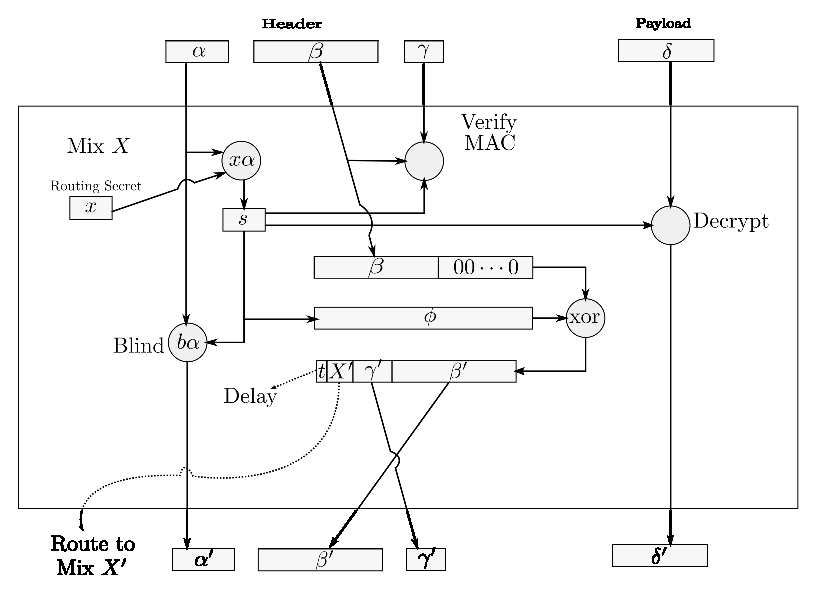
\includegraphics{sphinx1.eps}
  \end{center}
  \caption{The Sphinx packet format (reproduced from~\cite{Sphinx}).}
  \label{fig:sphinx}
\end{figure}

A Sphinx packet (Figure~\ref{fig:sphinx}) flows along a client-selected
route $X_1,\ldots,X_n$ where $n$ is less than some small network defined
constant.  A Sphinx packet consists of an elliptic curve point $\alpha$,
a routing header $\beta$ of a fixed length $L$, a single-use reply block
a MAC $\gamma$ that authenticates the contents of $\beta$, and a body
$\delta$.  Both $\beta$ and $\delta$ are onion encrypted, but $\beta$
uses a stream cipher, while $\delta$ uses a wide block cipher since
it is not authenticated.

Each hop $X$ processes $(\alpha,\beta,\gamma,\delta)$ as follows.  
First, it computes a shared secret $s = x \alpha$ to
derive a replay code, a MAC key, a stream cipher key, 
 a blinding key $b$, and a wide block cipher key. 
It uses the MAC key to check the MAC of $\beta$ and
 then checks its database for the replay code.
It aborts and drops the packet if either the MAC check fails or
 if the replay code is present.  Otherwise it adds the replay code
 to its database.
Next, it pads $\beta$ with $l$ zeros and decrypts the result
 using the stream cipher to produce a $\hat\beta$.
An initial segment of $\hat\beta$ of length $l' < l$ must contain
a valid routing command.  

We discuss some new routing commands in this paper, but the typical
routing command states the next hop $N'$ to which to forward the
packet, and the $\gamma'$ the next hop $N'$ requires. 
In this case, our hop $N$ computes $\alpha' := b \alpha$,
extracts $\beta' := \hat\beta[l'..L+l']$, and
decrypts $\delta$ using the wide block cipher to produce $\delta'$.
Now the packet $(\alpha',\beta',\gamma',\delta')$ is forwarded to $N'$,
 according to whatever mixing rules the protocol specifies.


\subsection{Cross over points}\label{subsec:crossover}

% FIXME: needs a diagram ;-).

A classical mix node command tells the mix to act as a ``cross over''
point by replacing the Sphinx header with a SURB stored in the packet.
We expect the recipient had previously supplied this SURB to the
sender, along with information like the cross over point from which
the SURB works, so this gives the recipient control over routing, 
and provides them with anonymity, even from the sender.  
The sender selects the path to the cross over point, so they can be
anonymous too, even from the recipient.
% TODO: Citation for cross over points?

A {\tt cross over} command provides a length $k$ along with new
 $\alpha''$ and $\gamma''$ that replace our old ones. 
We replace $\beta$ with $\beta'' := \beta'[0..k]$, or equivalently
$\hat\beta[l'..l'+k]$, followed by $L-k$ zero bytes.
\[ \beta'' :=  \beta'[0..k] \,||\, 0\cdots0 \]
In addition, $\delta$ is replaced by the decrypted $\delta'$, 
Now the mix reruns the Sphinx decoding process on the new packet
$(\alpha'',\beta'',\gamma'',\delta')$. 
After this second run there is nothing about the packet that 
identifies it --- not even to the original sender.
We zero the trailing $L-k$ bytes of $\beta''$ before decoding so that
the recipient can compute the required MACs, including $\gamma''$.

As stated, our recipient has chosen the cross over point $X$,
supplied the sender with $(X,\alpha'',\beta'[0..k],\gamma'')$,
and the sender built a route to $X$.  We imagine $\alpha$ to be
twice the size of $\gamma$ and $\gamma$ to be roughly the length of
$X$, so the {\tt cross over} command itself consumes 1.5 hops of $\beta$.
As the recipient picked $X$, this reduces the sender's maximum route
length by roughly 2.5 hops, plus any hops in $\beta''$.
We must bound the length $k$ or else the recipient could prevent
the sender from adding enough hops themselves, what we call a
long SURB attack.

\smallskip 

We could increase the total route length by one if we added a next
hop $X''$ to the {\tt cross over} command, built the tail of $\beta''$
using a stream cipher and sent $(\alpha'',\beta'',\gamma'',\delta')$
to $X''$. We consider this is wasteful because hops cost vastly more
than a few bytes in the header.

Worse, we observe that $\delta'$ has been stripped of all onion
encryption layers created by the sender because the sender must not
know anything about the packet after the cross over point,
 including wide block cipher keys.
We therefore forbid $\delta'$ from being the plaintext message itself
and insist that it be protected with another layer of end-to-end
encryption.  Indeed, this end-to-end encryption layer must use
different ephemeral keys to prevent cross over points from performing
correlation attacks on $\delta'$.

If all SURBs are supplied to the sender by the recipient, then
we could simply provide an extra wide block cipher key with which
the sender pre-encrypts $\delta$ before applying its own onion layers.
We do not assume this because SURBs have a limited lifespan though.  
If the sender does not posses any SURBs, then they could contact the
recipient through a {\em contact point}, and ask for SURB. 
These contact points would act like cross over points, except
that they would supply the SURB themselves from a stash supplied by
the recipient.

In this scenario, it impacts our mix networks' security less if
$\delta'$ is only ever seen by the cross over point, thereby
simplifying our overall design.   In particular, we might not mind
if the cross over point observes an ephemeral elliptic curve point
in $\delta'$, but even tools like Elligator~\cite{elligator} do not
conceal this point from a second hop.

In short, if we added this second hop $X''$ to lengthen the route
then $X''$ might discover its position as the hop after a cross over
point.  We could have a more oblivious hop at the cost of adding a
few bytes to the header.

\smallskip

There are two alternative approaches to encoding the SURB in the 
packet:  

First, the SURB could be placed into a special segment called
$\epsilon$, thus avoiding the long SURB attack check.
We must now however MAC $\epsilon$ like $\beta$ or else any
node in the sender's route can ``tag'' a message allowing its
identification by the cross over point $X$.  We also zero
$\epsilon$ at the cross over point like we zero the trailing
$L-k$ bytes of $\beta''$ currently.  We think placing the SURB
into $\beta$ buys us greater flexibility since $\epsilon$ has become
functionally equivalent to more $\beta$.

Second, we could place the SURB into a prefix of $\delta'$ because,
as noted above, $\delta'$ has been stripped of all onion encryption
layers created by the sender.  In this approach, a packet supports
a slightly larger payload if it does not use a SURB and perhaps
multiple SURBs for multiple recipients, so called garlic encryption.
In the short term, we fear that exploiting these options complicates
our API however.  Also, this scheme complicates the layering of
message and mix encryption.  We shall leave the door open for this
approach in future though becuase suport for multiple SURBs remains
an interesting option.


% \subsection{Sphinx packet construction}

% TODO: briefly explain packet construction ...


